\subsection{Muon triggers}
\label{sec:reco-mu-triggers}

Muons are triggered on at L1 using the RPC in the barrel (\modetalt{1.05}) and
the TGC in the endcaps (\modetalt{2.4}). As shown in~\fig{mu-trigger-diag}, the
muon trigger chambers are arranged in three planes of two to four layers; the L1
trigger fires on coincident hits in different planes. The coverage is $\sim$99\% in the
endcaps but only $\sim$80\% in the barrel due to gaps for services and the
detector feet.  The RPC planes consist of doublets of independent layers, and
for low \pt\ triggers a coincidence in 3 of 4 the four layers of the 2 inner planes
is required. The high \pt\ triggers start from the low \pt\ triggers, and look
for hits in one of the two layers of the third plane (referred to as the high
\pt\ confirmation plane). Similarly, the two outermost planes of the TGC consist
of doublets of independent detectors and low \pt\ triggers require the
coincident hits in 3 out of 4 layers. The TGC inner plane has 3
layers; high \pt\ triggers require coincidences in at least 2 out of the 3 layers
of this plane, in addition to the coincidences of a low \pt\ trigger. Coincidences are generated
separately for $\eta$ and $\phi$; a coincidence is required in both co-ordinates
for the trigger to be fired. To apply a \pt\ threshold to the trigger the
coincidences are required to fall inside \intro{roads}, parameterised
geometrical regions corresponding to muons of either charge with momentum above
a given \pt\ threshold. In 2011 the L1 \pt\ threshold for the primary single
muon trigger was 15 \GeV; in 2012 it was 20 \GeV.

\begin{figure}[h]
\centering
            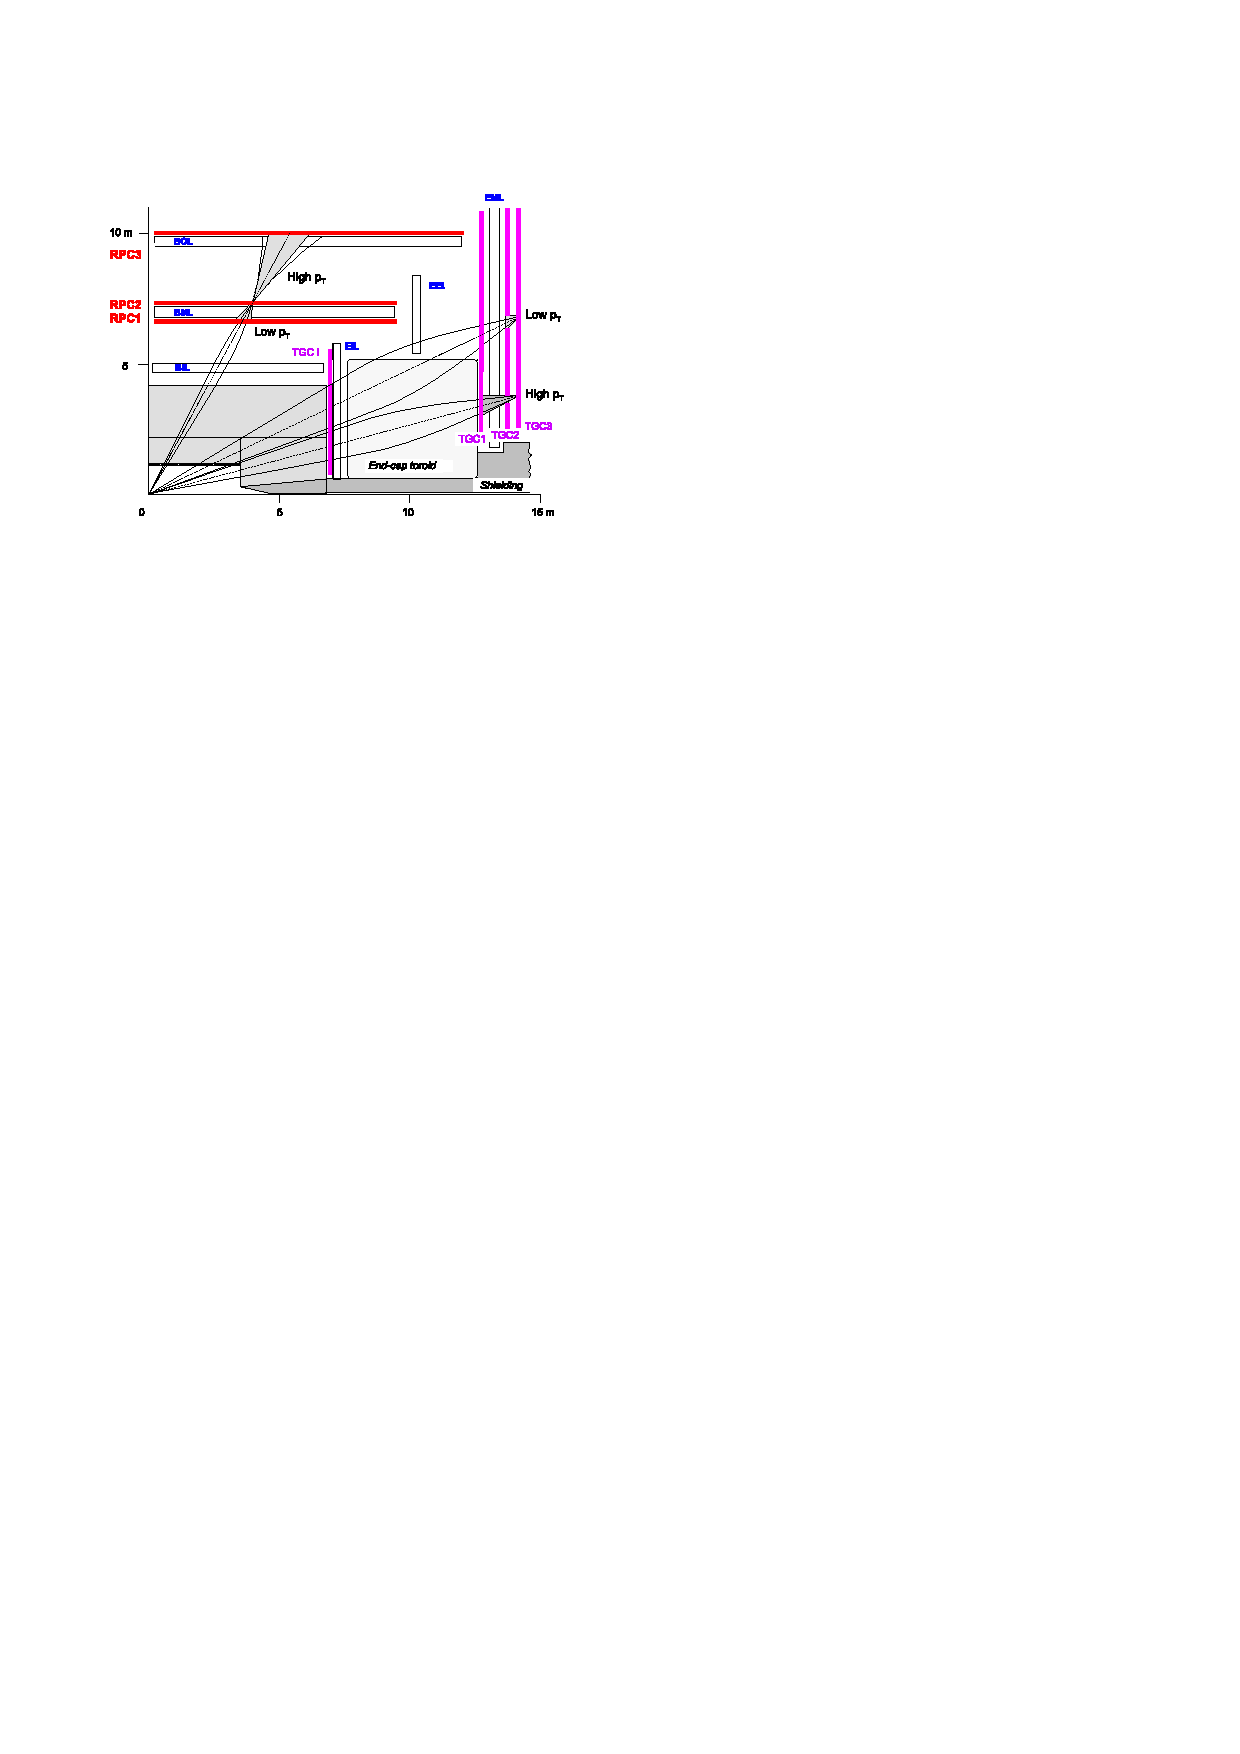
\includegraphics[width=0.8\textwidth]{mu-trigger-diag}
\caption{
Cross sectional view of the muon trigger chambers. Figure from~\cite{Aad:2012xs}.}
\label{fig:mu-trigger-diag}
\end{figure}

The muon HLT uses similar algorithms to the online muon reconstruction described
below. At L2, each L1 muon candidate is refined by including precision hit data
from the MDTs and CSCs in a RoI defined by the L1 candidate. MS tracks are
built by opening narrow roads around the L1 trigger chamber hits and associating
hits from other chambers to the track. A rough \pt\ measurement is obtained
using a lookup table. The MS tracks are then combined with ID tracks,
reconstructed using the same fast L2 ID tracking as the electron L2 trigger
(see~\sec{reco-el-triggers}). The muon EF uses the full offline algorithms,
running in RoIs determined by the L2 trigger. There are two reconstruction
strategies used at EF level: \intro{outside-in} (starting from the reconstructed
MS tracks, extrapolating to the beamline and attempting to combine with an ID
track) and \intro{inside-out} (starting from ID tracks and attempting to
extrapolate to the MS). In 2011, both strategies were ran in parallel to
maximise efficiency. In 2012, to reduce processing time, the outside-in
algorithm is run first, and only in events failing the trigger at this stage is
the inside-out algorithm run. In 2011 the HLT threshold used for the primary
single muon trigger was 18 \GeV; in 2012 it was raised to 24 \GeV. The muon
trigger is not sensitive to pile-up, but modifications were required in 2012 in
order to keep the rate at an acceptable level in the higher luminosity
conditions. To achieve this a track based isolation cut was applied at EF level,
requiring that the sum of the \pt\ of tracks in a cone of \deltaRlt{0.2} around
the muon track be less than 12\% of the muon's \pt. Only tracks with \ptgt{1}
enter the calculation, and to reduce pileup dependency, must have $|\Delta
z_{0}| <$ 6mm, where $\Delta z_{0}$ is the difference in longitudinal impact
parameter between the track and the muon track.

\subsection{Reconstruction and Identification}
\label{sec:reco-el-reco}

Muon reconstruction is in general based on combinations of accurate measurements
in the Muon Spectrometer and the Inner Detector~\cite{ATLAS-CONF-2010-064,ATLAS-CONF-2011-063}. There are four categories of
muons:

\begin{itemize}

    \item {\bf Combined:} combination of an MS track with an ID track. In
    general limited by the acceptance of the ID, \modetalt{2.5}, but due to the complicated
    nature of the magnetic field it is possible to get combined muons beyond
    this.

    \item {\bf Segment Tagged:} combination of an ID track with an MS track
    segment. An MS track segment is a straight line track segment reconstructed
    in a single MS station where the segment did not form a full MS track. The
    track parameters of the reconstructed muon are taken solely from the ID
    track.

    \item {\bf Stand Alone:} muon track reconstruction based solely on 
    MS measurements. Possible over the full acceptance of the MS,
    \modetalt{2.7}.

    \item {\bf Calorimeter Tagged:} ID tracks are tagged as originating from
    muons by matching them to calorimeter deposits consistent with a minimum ionising
    muon. No MS information is used.


\end{itemize}

Since combined muons have a fully reconstructed track in both the ID and the MS
they are the preferred muon type and will have the best track parameter
resolution. The ID provides the best momentum measurement at low to intermediate
momenta, whereas the MS provides the better measurement at higher \pt\ (roughly
for \ptgt{100}). Combination with an ID track improves the momentum resolution
over the range $4 < p_{T} < 100$ \GeV. Segment tag muons are useful to recover
efficiency at low \pt\ where muons may only reach the inner layer of the muon
chamber and in regions of limited detector acceptance. Stand alone muons are
useful to extend coverage beyond the coverage of the ID. Calorimeter tagged
muons suffer large fake rates from jets and electrons, but can be used to recover
acceptance at \modetalt{0.1} where there are gaps in the muon chambers to
provide space for services to the ID, the solenoid magnet and the calorimeters.

There are two parallel muon reconstruction chains in use in ATLAS,
\staco\cite{1742-6596-219-3-032052} and
\muid. Each use slightly different track finding algorithms, and approach the
combination of ID and MS tracks in different ways. \muid\ performs a global
refit of hits in the MS and the ID, whereas \staco\ attempts a statistical
combination of the two track measurements, weighting the relative contributions
according to their covariance matrices. The two chains are found to give similar
performance (see ??). The measurements in this thesis all use muons
reconstructed with the \staco\ chain, so this chain is described in detail here.

The \staco\ chain begins with the reconstruction of MS tracks using the \muonboy\
algorithm. First, the muon trigger chambers are used to identify Regions of
Activity (RoA). The RoA are areas of size \deltaetadeltaphi{0.4}{0.4} where
there is at least one RPC or TGC hit in both co-ordinates. Local straight track
segments are then reconstructed within the RoA by attempting to combine each MDT
hit in a multilayer with each MDT hit in the other multilayer of the same or
adjacent station. This gives four possible track segments. Each of these segments
is extrapolated to the rest of the MDT tubes and matched with hits. The segment candidates are required to point loosely towards the
interaction point, and cuts are applied on the \chisquared\ of the track
segment, with penalties for missing hits. 

Track candidates are then formed by combining at least
two segments from different stations to form track candidates. The tracks are
seeded from track segments that have at least one second-coordinate hit. A first
rough estimate of the momentum is deduced from the position and direction of the
segment. Each of these segments is then extrapolated to the other stations, and
matches in position and direction is found. Since the track momentum is not well
known at this point, a `momentum-scan' of several possible momentum values is
performed. The best match (if any) is chosen, and the track segments are
combined and refitted to obtain a more accurate momentum measurement. A second,
finer momentum scan is performed around the improved momentum estimate,
extrapolating to all other stations, including ones which match to the track.
The track is then refit (still using the track segments as inputs) to more accurately determine the momentum, position and
direction. 

Then, a global fit is performed on the candidate tracks, starting from the
best results of the previous fit, but using the raw hit information. This gives
a better estimate of the likelihood of the track and gives a better
discrimination of outlier hits from `good' hits. Finally, a last fit including
a detailed description of the material traversed by the tracks is performed.
this fit properly takes into account multiple scattering effects, and the
scattering angles at a set of discretised scattering centres are included in the
fit. The energy loss due to interactions is also taken into account  by
parametrising the most probable energy loss as as a function of the track momentum and
the amount of material crossed. The selection of reconstructed muons is made
based on the \chisquared\ quality of this final fit.

Selected muon tracks are then extrapolated back to the interaction point,
correcting for energy loss and multiple scattering in the calorimeters and the
material of the ID~\footnote{The typical energy loss in the calorimeter is $\sim
3$ \GeV.}. MS tracks are then combined with ID tracks by selecting tracks to be
paired on the basis of a match \chisquared, defined from the difference between
the two sets of track parameters weighted by their combined covariance matrix.
The track parameters are combined, weighting the relative contributions
according to their covariance matrix.

The efficiency of the muon reconstruction in the MS decreases very rapidly with
decreasing \pt\ because accurate tracking of low \pt\ muons in the highly
inhomogeneous magnetic field is very complicated.
Furthermore as \pt\ decreases, the energy lost by the muons inside the
calorimeters becomes comparable to their energy, especially in the barrel
region. The \mutag\ algorithm is used to recover efficiency at low \pt\ by
starting from ID tracks, extrapolating them to the inner station of the MS and
attempting to match them with MS track segments not yet associated to combined
tracks.

\subsubsection{Calorimeter Tagged Muons}

It is also possible to reconstruct muons independently of the MS by using the calorimeter to tag inner-detector tracks originating from muons.
 A muon
with sufficient momentum will traverse all layers of the calorimeter,
leaving a small energy deposit in each layer. It is possible to distinguish this
pattern of energy deposition from that of other particles. A low
momentum hadron will deposit most of its energy in the first layers of the
calorimeter, leaving no signal in the last layers. High momentum hadrons will
deposit most of their energy in the core cells, and electrons will deposit most of their energy
in the EM calorimeter. The \CaloTrkMuID\ algorithm identifies muon candidates by
requiring an ID track matched to a signal consistent
with a minimum-ionising-particle in each layer of the
calorimeter. 
 %to reject hadron and electron backgrounds
Both a cut based quality selection and a likelihood
ratio based quality selection are used, and muon candidates passing either are
accepted. Calorimeter tagged muons are used to recover efficiency at
\modetalt{0.1} where there is a gap in the muon-spectrometer.

\subsubsection{Reconstruction efficiencies}

~\fig{el-reco-eff} shows the observed reconstruction efficiency, measured using
a tag and probe method on Z boson decays~\cite{ATLAS-CONF-2011-063}, for Combined and Segment
Tagged muons in the 2011 data, as well as the efficiency predicted by the
Monte-Carlo simulation. The efficiency is
seen to drop significantly for \modetalt{0.1} for reasons explained above. The
efficiency for calorimeter tagged muons is also shown, and it is seen that this
effectively recovers the loss in efficiency at \modetalt{0.1}. The muon
reconstruction efficiency is seen to be almost constant as a function of \pt. In
both \pt\ and $\eta$ good agreement is seen between the simulation and the data,
but as with the electrons, scale-factors are applied to the Monte-Carlo to
reproduce the efficiency observed in data.

\begin{figure}[h]
\centering
	\subfigure[]{
            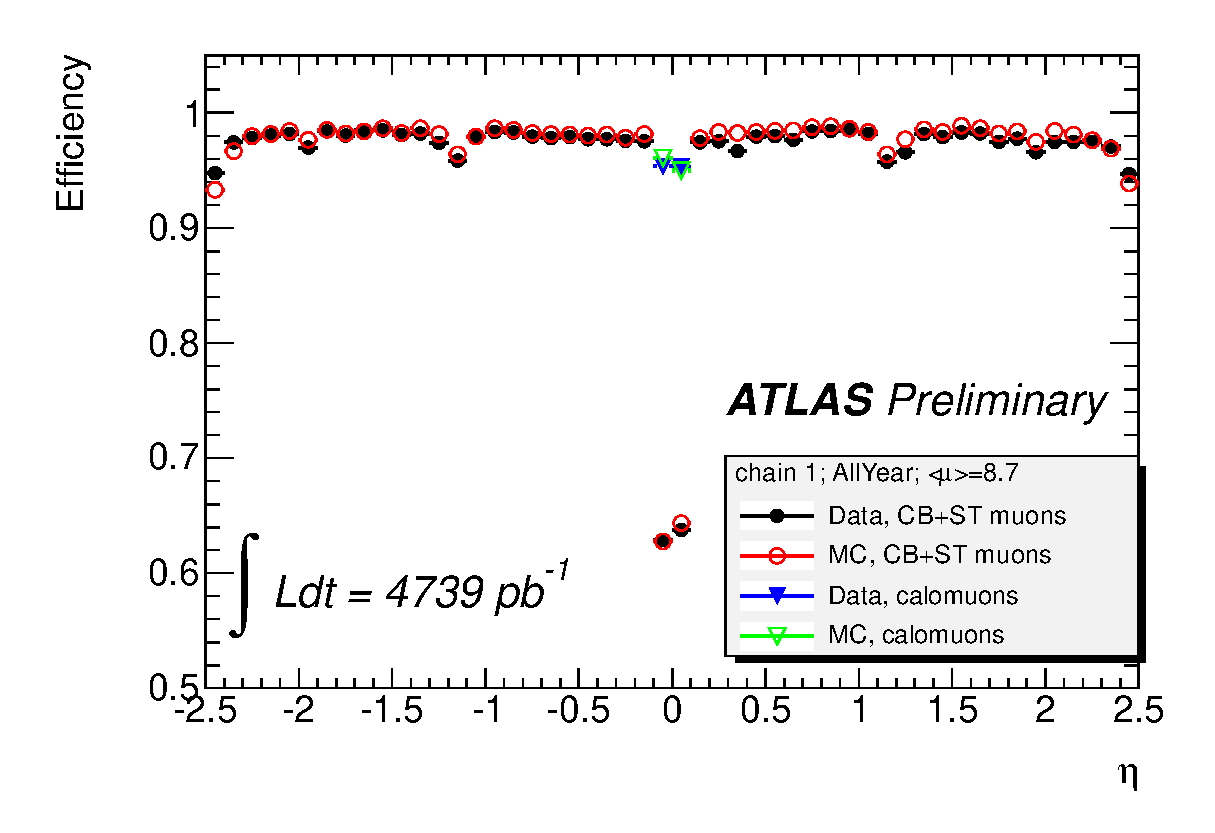
\includegraphics[width=0.475\textwidth]{STACO_loose_id_vs_eta}
        }
	\subfigure[]{
            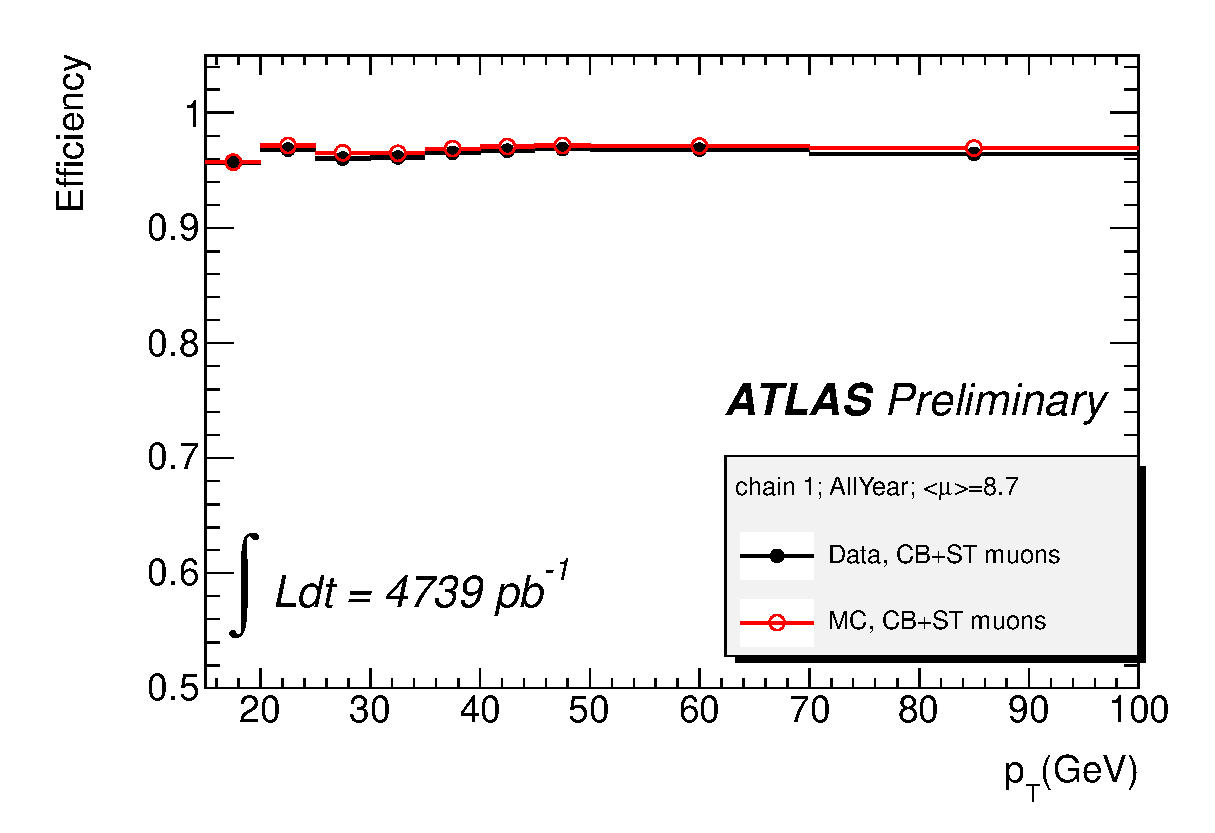
\includegraphics[width=0.475\textwidth]{STACO_loose_id_vs_pt}
        }
\caption{Muon reconstruction efficiency in 2011 as a function of (a) the pseudorapidity
and (b) the transverse momentum of the muon for either Combined or Segment
Tagged muons reconstructed using the \staco\ algorithm. The solid black points
show the efficiency observed in data, and the open red circles show the
efficiency predicted by Monte-Carlo simulation. In figure (a) the efficiencies for
calorimeter tagged muons are also shown for \modetalt{0.1} (solid blue triangles
for data and open green triangles for Monte-Carlo). Figures from~\cite{MuonEfficiency2011}.}
\label{fig:mu-reco-eff}
\end{figure}


% each station consists of two layers of MDT sandwiched between RPC chambers





